% Project Topic Proposal — Shift-Left Accessibility (minimal emphasis)
\documentclass[12pt]{article}
\usepackage[left=1in,right=1in,top=1in,bottom=1in]{geometry}
\usepackage{setspace}
\usepackage{graphicx}
\singlespace

\title{Shift-Left Accessibility for UX/UI: A Figma Preflight vs.\ Code-Time Checks (Pilot)}
\author{Noelynn Faith Batalingaya}
\date{September 2025}

\begin{document}
\maketitle

\section*{Problem Statement \& Motivation}
My project asks a practical question: how much accessibility can we catch while the interface is still a Figma mockup, and does doing that early save time once we write code? In real teams, accessibility often shows up late and creates rework. I will test whether a short, repeatable “preflight” checklist during design reviews prevents common issues from ever reaching implementation.

\section*{Background \& Prior Work}
Accessibility is about real people being able to use what we ship—from screen reader and keyboard-only users to people with low vision, older adults, and anyone using a cracked phone outdoors. HCI research argues that inclusive design should start at the beginning, not as a last-minute checklist \cite{bennett2018inclusive}. Recent studies show that many problems are visible in the mockups themselves—low color contrast, small hit targets, unclear component states, and weak hierarchy—and can be assessed systematically in Figma before any code exists \cite{huang2024a11yfigma, chen2024figmaapps}. Work with UX practitioners also highlights barriers such as time, ownership, and uneven training, and recommends lightweight checklists and design-system constraints as realistic improvements \cite{shi2023uxaccesspractice}. This pilot turns those insights into a small but measurable study.

\section*{Project Scope \& Goals}
Goal 1. Create a one-page Figma Accessibility Preflight centered on five checks: (a) contrast and legibility, (b) hierarchy and structure, (c) target size and spacing, (d) state visibility (focus/hover/active/disabled/error), and (e) basic semantics and affordances (labels, recognizable controls).\\
Goal 2. Implement two matching screens (Home and Register) as a tiny website and run code-time checks (keyboard, screen reader, automated tools).\\
Goal 3. Compare which issues are caught when, and the minutes to fix at design versus code time.

Research Questions. RQ1: Which issue types are reliably caught at design time versus only at code time (for example, focus order and announcements)? RQ2: Does the preflight reduce minutes to fix compared to fixing after implementation?

\section*{Planned Software (what I will build)}
To keep effort manageable and the focus on accessibility (not tooling), I will build a minimal two-page site using HTML/CSS with a small amount of JavaScript:
\begin{itemize}
  \item Home: semantic landmarks (\texttt{header/nav/main/footer}), a visible “Skip to main content” link, proper headings, high-contrast tokens, and a clear \texttt{:focus-visible} outline.
  \item Register: explicit \texttt{<label for>} on each field, hint text via \texttt{aria-describedby}, inline error messages with \texttt{role="alert"}, and focus moves to the first error on submit. All key interactions work by keyboard (Tab/Shift-Tab/Enter/Space/Esc).
\end{itemize}

\section*{Method \& Measures}
Phase A — Design-time preflight. I will run the five checks on two Figma mockups (Home, Register). For every issue, I will log: \texttt{screen\_id}, phase=design, category, severity, found\_by=preflight, fix\_minutes, notes. Then I will update the mockups and record design fix minutes.

Phase B — Code-time checks. I will build the two pages and perform three passes:
\begin{enumerate}
  \item Keyboard pass: reach everything with Tab/Shift-Tab, visible focus, no traps, expected Enter/Space/Esc behavior.
  \item Screen reader pass (macOS VoiceOver): names/roles/labels, headings/landmarks, and whether errors are announced.
  \item Automated audits: Lighthouse and axe DevTools for quick, repeatable checks.
\end{enumerate}
Each issue will be logged with phase=code and code fix minutes.

Analysis. I will compare counts by phase and category and graph the average minutes to fix at design versus code. Based on prior work, I expect the preflight to catch many visual and structural issues quickly, while code-time checks remain essential for focus order and screen reader announcements \cite{huang2024a11yfigma, chen2024figmaapps, shi2023uxaccesspractice}. I will note limits (small pilot, student context) and outline how to expand next semester (more screens; possibly recruit assistive technology users; compare teams with versus without the preflight).

\section*{Illustration (logic only)}
This proposal includes one figure: a logic diagram summarizing the flow from the Figma preflight to code-time checks and the final comparison of issues and fix minutes (Figure~\ref{fig:logic}).

\begin{figure}[h]
  \centering
  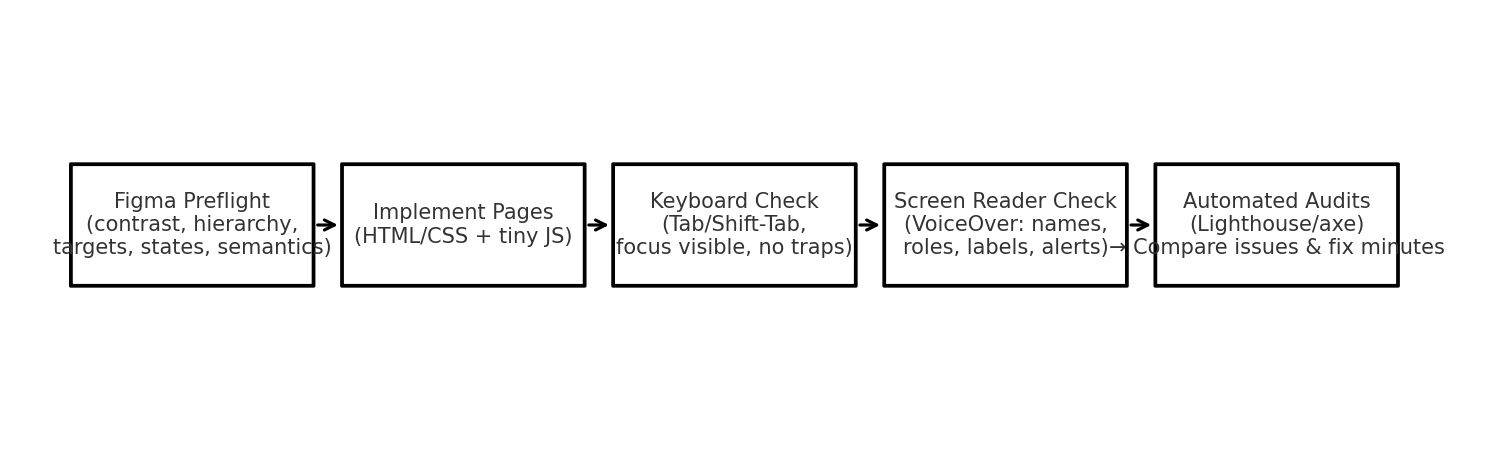
\includegraphics[width=0.95\linewidth]{imgs/logic-diagram.png}
  \caption{Workflow: Preflight on mockups $\rightarrow$ implement pages $\rightarrow$ keyboard/screen reader/axe checks $\rightarrow$ compare issues and fix minutes.}
  \label{fig:logic}
\end{figure}

\section*{Expected Contributions}
Deliverables will include: (1) a short, printable preflight that can be used in design critique, (2) a small set of accessible component patterns (focus ring, skip link, labeled inputs, reduced motion), and (3) a small dataset showing where early checks save time and where code-time checks are still required. These are practical outcomes for student teams and a foundation to scale into a larger Senior IS.

\newpage
\section*{Appendix: Feature List (implementation order)}
\begin{enumerate}
  \item Add semantic landmarks and a “Skip to main content” link.
  \item Set heading hierarchy (H1/H2/H3) and spacing scale.
  \item Add a clear \texttt{:focus-visible} outline (high contrast, offset).
  \item Define color tokens and verify contrast (text and UI) against WCAG AA.
  \item Build Home navigation: keyboard-reachable links; hover/active states; visible focus.
  \item Build Register form with \texttt{<label for>} and hint text via \texttt{aria-describedby}.
  \item Inline error message with \texttt{role="alert"} and focus-to-first-error on submit.
  \item Enforce target size minimums (about 44×44 px) and adequate spacing between controls.
  \item Respect \texttt{@media (prefers-reduced-motion)} for users who limit animation.
  \item Run Lighthouse/axe; log issues and \texttt{fix\_minutes}; capture before/after screenshots.
  \item[\textit{Stretch}] Add a basic table pattern (caption, header cells with scope) plus a one-sentence text summary.
  \item[\textit{Stretch}] Add a short alt-text guide and test a tiny image gallery (good versus poor examples).
  \item[\textit{Stretch}] Optional automation: run Pa11y or jest-axe locally for quick regression checks.
\end{enumerate}

\nocite{bennett2018inclusive, huang2024a11yfigma, chen2024figmaapps, shi2023uxaccesspractice}

\clearpage
\bibliographystyle{acm}
\bibliography{bibliography}
\end{document}
